\documentclass[a4paper,11pt,titlepage]{article}
% The maths package
\usepackage{amsmath}
\usepackage{amsfonts}
% The graphics package
\usepackage{graphicx}
% Allows paragraph in blocks
\usepackage{parskip}
% Code hightling
\usepackage{minted}
% Verbatim file inclusion
\usepackage{fancyvrb}

%%%% Define the title %%%%%%%%%%%%%%%%%%%%%%%%%%%%%%%%%%%%%%%%%%%%%%%%%%%%%%%%%%
\title{
MECH3750 Engineering Analysis II \\ 
Assignment 2
}
% define the author
\author{
Merrick Heley\\
42339915
}

%%%% Notes, commands, settings %%%%%%%%%%%%%%%%%%%%%%%%%%%%%%%%%%%%%%%%%%%%%%%%%
% \section*{Task 1} uses an asterisk to suppress the section number

% This command adds \ud for finishing integrals
\newcommand{\ud}{\,\mathrm{d}}

% Set the pygmentation style for code
% pygmentize -L styles
\usemintedstyle{autumn}

% Simple command for python file input
\newcommand{\inputpython}[1]{
    \inputminted[linenos=true, 
                 frame=single, 
                 fontsize=\scriptsize, 
                 label=#1]
                {python}{#1}
}

% Simple command for python file output
\newcommand{\pythonoutput}[1]{
    \immediate\write18{python #1 > #1.out}
    \fvset{frame=single, numbers=left, fontsize=\scriptsize, label=#1.out}
    \VerbatimInput{#1.out}
    \write18{del #1.out}
}

% Simple command for python file input
\newcommand{\inputmaxima}[1]{
    \inputminted[linenos=true, 
                 frame=single, 
                 fontsize=\scriptsize, 
                 label=#1]
                {cpp}{#1}
}

%%%% Start document %%%%%%%%%%%%%%%%%%%%%%%%%%%%%%%%%%%%%%%%%%%%%%%%%%%%%%%%%%%%

\begin{document}
% generates the title
\maketitle

%%%% Question 0.1 %%%%%%%%%%%%%%%%%%%%%%%%%%%%%%%%%%%%%%%%%%%%%%%%%%%%%%%%%%%%%%
\section*{Question 0.1: Boundary Value Problems}
\subsection*{a. Shooting Method}

\subsection*{b. Lehmer-Shur Algorithm}

\subsection*{c. Difference Method}

\begin{align}
-y'''(x) + y''(x) - 4xy'(x) + (8x + 3)y(x) &= x^2 \label{eq:q1bvp}\\
y(-1) & = -10 \notag\\
y(0.5) & = 1 \notag\\
y(1.5) & = -3 \notag
\end{align}

To solve this boundary value problem using difference method, approximations 
must be formed using a difference approximation. To keep the problem simple, a 
first order central difference method was initially used.

\begin{align}
y' & = \frac{1}{2h}(y_{i+1} - y_{i-1}) \label{eq:central1}\\
\intertext{When this equation is substituted into itself, it can be derived 
            further}
y'' & = \frac{1}{h^2}(y_{i+1} - 2y_i + y_{i-1}) \label{eq:central2}\\
\intertext{And once more}
y''' & = \frac{1}{2h^3}(y_{i+2} - 2y_{i+1} + 2y_{i-1} - y_{i-2}) 
            \label{eq:central3}
\intertext{Substituting \eqref{eq:central1} \eqref{eq:central2} \eqref{eq:central3} 
            into \eqref{eq:q1bvp}}
x_i^2 & = -\frac{1}{2h^3}(y_{i+2} - 2y_{i+1} + 2y_{i-1} - y_{i-2}) \notag\\
      &   + \frac{1}{h^2}(y_{i+1} - 2y_i + y_{i-1}) \notag\\
      &   - \frac{4x}{2h}(y_{i+1} - y_{i-1}) \notag\\
      &   + (8x + 3)y_i \\
\intertext{And rearranging to group $y_i$ values together}
x_i^2 & = \left(\frac{1}{2h^3}\right)y_{i-2} + \notag\\
      & \left(\frac{-2}{2h^3} + \frac{1}{h^2} + \frac{4x}{2h}\right)y_{i-1} + \notag\\
      & \left(\frac{-2}{h^2} + (8x + 3)\right)y_i + \notag\\
      & \left(\frac{2}{2h^3} + \frac{1}{h^2} + \frac{-4x}{2h}\right)y_{i+1} + \notag\\
      & \left(\frac{-1}{2h^3}\right)y_{i+2} \label{eq:bvpcentral} \\
\intertext{This equation is modelled in the function 'f(x, h)' in the code}
\intertext{It can be seen in \eqref{eq:bvpcentral} that at the first and final
            steps, an invalid value will be referenced (e.g. at -0.9, $y_{i-2}$
            will correspond to -1.1, at which we have no data). To handle this,
            \eqref{eq:central2} will be derived using a forward difference 
            method rather than a central difference method.}
\intertext{The forwards difference approximation is}
y' & = \frac{1}{h}(y_{i+1} - y_i) \label{eq:forward1}\\
\intertext{And deriving \eqref{eq:central2} with \eqref{eq:forward1} gives}
y''' & = \frac{1}{h^3}(y_{i+2} - 3y_{i+1} + y_i - y_{i_1}) \label{eq:forward3}\\
\intertext{Substituting \eqref{eq:central1} \eqref{eq:central2} \eqref{eq:forward3}
            in to \eqref{eq:q1bvp} and rearranging to group $y_i$ values together}
x_i^2 & = \left(0\right)y_{i-2} + \notag\\
      & \left(\frac{1}{h^3} + \frac{1}{h^2} + \frac{4x}{2h}\right)y_{i-1} + \notag\\
      & \left(\frac{-3}{h^3} + \frac{-2}{h^2} + (8x + 3)\right)y_i + \notag\\
      & \left(\frac{3}{h^3} + \frac{1}{h^2} + \frac{-4x}{2h}\right)y_{i+1} + \notag\\
      & \left(\frac{-1}{h^3}\right)y_{i+2} \label{eq:bvpforward}\\
\intertext{This equation is modelled in the function 'fForward(x, h)' in the code}
\intertext{Using the backwards difference approximation}
y' & = \frac{1}{h}(y_{i} - y_{i-1}) \label{eq:backward1}\\
\intertext{and a similar process to the forward difference method, the final 
            grouped $y_i$ values with the backwards difference method subbed 
            in are}
x_i^2 & = \left(\frac{1}{h^3}\right)y_{i-2} + \notag\\
      & \left(\frac{-3}{h^3} + \frac{1}{h^2} + \frac{4x}{2h}\right)y_{i-1} + \notag\\
      & \left(\frac{3}{h^3} + \frac{-2}{h^2} + (8x + 3)\right)y_i + \notag\\
      & \left(\frac{-1}{h^3} + \frac{1}{h^2} + \frac{-4x}{2h}\right)y_{i+1} + \notag\\
      & \left(0\right)y_{i+2} \label{eq:bvpbackward}
\intertext{This equation is modelled in the function 'fBackward(x, h)' in the code}\notag
\end{align}
To generate a solution to this equation, it is necessary to solve the equation
\begin{equation}
JY = X
\end{equation}
Where $J$ is the $n \times n$ system of equations for the LHS of the system, 
$X$ is the $n \times 1$ matrix of the RHS of the system
and $Y$ is the set of $y$ values at each point on $X$.

As the step size is known (at 0.1) a 26x26 matrix can be made (the code is 
invariant to this step size, however significantly increasing it will slow 
the execution time) and can be populated along its diagonal using the central 
difference method. In cases where the central difference method will attempt to 
use values outside the matrix (i.e. close to the edges of the matrix), forwards 
and backwards difference methods can be used (see line 155 ``\# Handle difference 
approximation at boundaries'' in the code

Finally, at x values where the solution is known (i.e. the boundary values), 
the element in the $X$ matrix corresponding to this point should be set to the 
known solution (see line 57 ``\# Handle boundary values'' in the code) and the 
corresponding row in the $J$ matrix should be set to all 0's with a single '1'
in it's diagonal element (see line 82 ``\# Handle boundary values'' in the code).

These generated matrices are shown in the output of the python code.

\inputpython{Task1c.py}
\pythonoutput{Task1c.py}

\begin{figure}[!hbp]
\centering
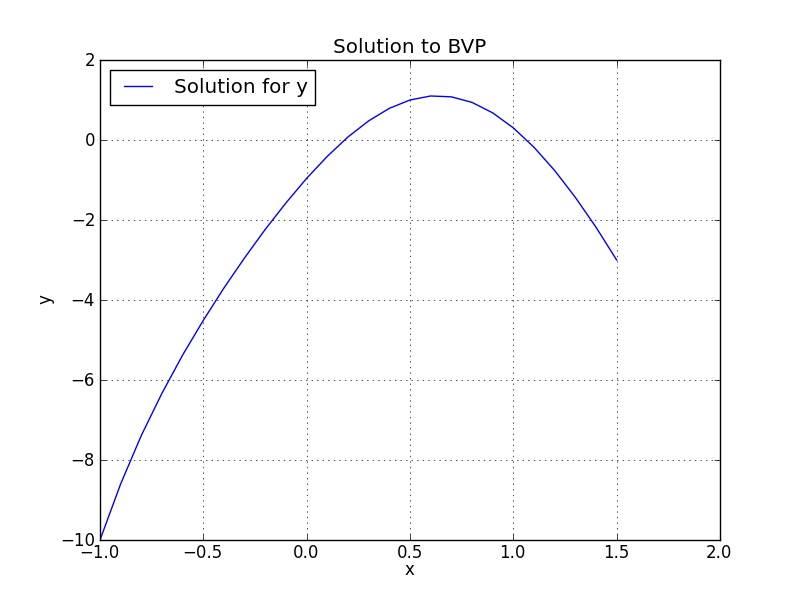
\includegraphics[scale=0.5]{Task1c.png}
\caption{Solution to BVP using Difference Method}
\end{figure}

It can be seen the solution using the difference method is extremely similar to 
the solution using the shooting method.

\subsection*{d. Non-Linear Difference Method}

%%%% Question 0.2 %%%%%%%%%%%%%%%%%%%%%%%%%%%%%%%%%%%%%%%%%%%%%%%%%%%%%%%%%%%%%%
\section*{Question 0.2: Newtons Method}
\subsection*{a. Single Solution}

\subsection*{b. Solutions in $\mathbb{C}$}

\subsection*{c. Proof of number of solutions}

\subsection*{d. Maxima Brute-force}
\inputmaxima{Task2d.wxm}

%%%% APPENDICES %%%%%%%%%%%%%%%%%%%%%%%%%%%%%%%%%%%%%%%%%%%%%%%%%%%%%%%%%%%%%%%%
\clearpage
\section*{Appendix A}
% Bisection method in appendix (shitty, and not correct way of doing appendices)
\inputpython{secant.py}
\pythonoutput{secant.py}



\clearpage
\end{document}